\documentclass{alex_hü}

\name{Alexander Helbok}
\course{PS Physik}
\hwnumber{5}


\begin{document}
\renewcommand{\labelenumi}{(\alph{enumi})}


\begin{mybox}{1. Kondensatornetzwerk}
	\centering \( C_1 = 450 \unit{nF};\quad C_2 = 300 \unit{nF};\quad C_3 = 600 \unit{nF};\quad C_4 = 100 \unit{nF};\quad U = 120 \unit{V} \)
	\tcblower
		\begin{flalign*}
			C_{ges} &= \tfrac{C_1\left( \tfrac{C_2C_3}{C_2+C_3} + C_4 \right)}{C_1 + \tfrac{C_2C_3}{C_2 + C_3} + C_4} = 180 \unit{nF} &&\\[1.5em]
			U_1 &= U \tfrac{C}{C_1} = \dl{48 \unit{V}} &&\\
			U_2 &= U_4 \tfrac{C_3}{C_3 + C_2} = \dl{48 \unit{V}} &&\\
			U_3 &= U_4 \tfrac{C_2}{C_2 + C_3} = \dl{24 \unit{V}} &&\\
			U_4 &= U - U1 = \dl{72 \unit{V}} &&
		\end{flalign*}
		\hfill
		\begin{minipage}[t]{0.5\textwidth}
			\vspace{-5.5cm}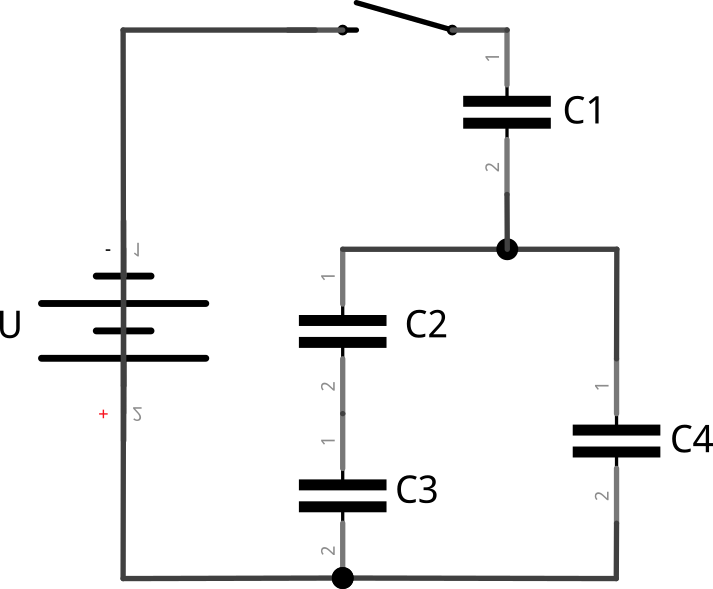
\includegraphics[scale=0.35]{Condens}
		\end{minipage}
\end{mybox}

\begin{mybox}{2. Wickelkondensator}
	\centering \( k = \tfrac{1}{4\pi \epsilon_0};\quad d = 2.0 * 10^{-5}\unit{m};\quad b = 0.02 \unit{m};\quad C = 100\unit{nF};\quad \epsilon = 2.3 \)
	\tcblower
	\begin{enumerate}
		\item \( \omega = \sqrt{\tfrac{mgl}{I}} \)
		\begin{flalign*}
			I &= \tfrac{1}{12}m(a^2 + h^2) + ml^2 = 0.12 \unit{kg.m^2} &&\\
			\omega_a &= \sqrt{\tfrac{mgl}{I}} = \dl{6.37 \unit{rad/s}} &&
		\end{flalign*}
	\tcbline
		\item \( F = -m\omega^2 x;\quad \Delta x = x_1 - x_2 \)
%		\begin{flalign*}
%	
%		\end{flalign*}
	\end{enumerate}
\end{mybox}

\begin{mybox}{3. Ladungsträger}
	\centering \(  \)
	\tcblower
	\begin{enumerate}
		\item \( r = 1.85 * 10^{-4} \unit{m};\quad I = 1 \unit{A} \)
		\begin{flalign*}
			n &= \tfrac{N_A\rho_{Cu}}{M_{Cu}} &&\\
			v_D &= \tfrac{I}{ne\pi r^2} = \dl{2.75 * 10^{-3} \unit{\v}} &&
		\end{flalign*}
	\tcbline
		\item \( L = 10 \unit{m} \)
		\begin{flalign*}
			t &= \tfrac{L}{v} = \dl{3630.97 \unit{s}} &&
		\end{flalign*}
	\tcbline
		\item A constant Potential means a constant Electric field
	\tcbline
		\item Drift velocity sinks when the conductor gets heated because a higher temperature means higher resistance. On a microscopic level this means that the electrons bump into more Obstacles and their path is more obstructed.
	\tcbline
		\item \( I = \tfrac{U}{R} = \tfrac{UA}{\rho L} \)
			\begin{enumerate}[label=\roman*.]
				\item \( I_1 = \tfrac{UA}{\rho L} \)
				\item \( I_2 = \tfrac{3}{4}\tfrac{UA}{\rho L} \)
				\item \( I_3 = \tfrac{UA}{\rho L} \)
			\end{enumerate}
			\( \Rightarrow \dl{I_2 < I_1 = I_3} \)
	\end{enumerate}
\end{mybox}

\begin{mybox}{4. Ladungstransport}
	\centering \( L = 1 \unit{m};\quad d = 0.001 \unit{m};\quad I = 1 \unit{A} \)
	\tcblower
	\begin{enumerate}
		\item \( R = \tfrac{L}{\sigma_{el}A} = \tfrac{U}{I};\quad \sigma_{el} = 6 * 10^7 \unit{\ohm/m} \)
		\begin{flalign*}
			R &= \tfrac{4L}{\sigma_{el}\pi d^2} = \dl{0.021 \unit{\ohm}} &&\\
			U &= RI = \dl{0.021 \unit{V}} &&
		\end{flalign*}
	\tcbline
		\item \( \rho = 9000 \unit{kg/m^3};\quad M = 0.064 \unit{kg/mol};\quad V = \tfrac{Ld^2\pi}{4} \)
		\begin{flalign*}
			n &= \tfrac{\rho N_AV}{M} = 6.62 * 10^{22} &&\\
			n_{el} &= n = \dl{6.62 * 10^{22}} &&\\[1em]
			v_D &= \tfrac{I L}{n_{el}e} = \dl{9.43 * 10^{-5} \unit{\v}} &&
		\end{flalign*}
	\tcbline
		\item \( \delta\omega = \omega_b - \omega_a \)
		\begin{flalign*}
			0 &= \cos(\tfrac{1}{2}\delta\omega t) &&\\
			t &= \tfrac{2\arccos(0)}{\delta\omega} = \dl{50.29 \unit{s}} &&
		\end{flalign*}
	\end{enumerate}
\end{mybox}

\end{document}